% Part: model-theory
% Chapter: interpolation
% Section: separation

\documentclass[../../../include/open-logic-section]{subfiles}

\begin{document}

\olfileid{mod}{int}{sep}

\olsection{د \printtoken{P}{sentence} بېلول}

د منځګړيتوب د قضيې ثبوت ته تر تلو مخکې لږ بنسټيز کار پکار دے۔ د
$!A$ او~$!B$ منځګړی داسې !!a{sentence}~$!C$ ده چې
$!A \Entails !C$ او $!C \Entails !B$ وي۔ د نقيض عکس له مخې،
وروستۍ خبره هله او يوازې هله رښتونې ده چې
$\lnot !B \Entails \lnot !C$ وي۔ هغه !!^a{sentence}~$!C$ چې دا
خاصيت ولري، ويل کېږي چې $!A$ او~$\lnot !B$ \emph{بېلوي}۔ نو د
$!A$ او~$!B$ د يو منځګړي موندل د داسې !!a{sentence} له موندلو سره
برابر دي چې $!A$ او~$\lnot !B$ بېل کړي۔ د معمول په څېر به د يوې
عمومي شوې بڼې څېړل ګټور وي: داسې جمله چې د !!{sentence}s دوه
\emph{سټونه} بېل کړي۔

\begin{defn}
يوه جمله~$!C$ د جملو سټونه~$\Gamma$ او~$\Delta$ هله او يوازې هله
\emph{بېلوي} چې $\Gamma \Entails !C$ او
$\Delta \Entails \lnot !C$ وي۔ که داسې هېڅ !!{sentence} نۀ وي،
نو~$\Gamma$ او~$\Delta$ \emph{نه بېلېدونکي} دي۔
\end{defn}

د~$\Gamma$، $\Delta$ او~$!C$ د مدلونو د ټولګيو تر منځ د شاملېدو
اړيکې لاندې ښودل شوې دي:
\begin{figure}[h]
  \centering
  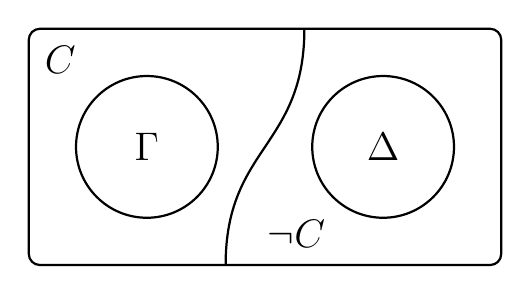
\begin{tikzpicture}[node distance=2cm, auto, thick]
    \draw [rounded corners] (0,0) -- (6,0) -- (6,3) -- (0,3) --  cycle;
    \draw (1.5,1.5) circle (0.9cm);
    \draw (4.5,1.5) circle (0.9cm);
    \path node at (1.5,1.5) {\Large $\Gamma$};
    \path node at (4.5,1.5) {\Large $\Delta$};
    \path node at (0.4,2.6) {\Large $\formula{C}$};
    \path node at (3.4,0.4) {\Large $\lnot \formula{C}$};
    \draw (2.5,0) .. controls (2.5,1.5) and (3.5,1.5) .. (3.5,3);
  \end{tikzpicture}
  \caption{$!C$، $\Gamma$ او~$\Delta$ بېلوي}
  \ollabel{fig:sep}
\end{figure}


\begin{lem}\ollabel{lem:sep1}
فرض کړئ~$\Lang{L}_0$ هغه ژبه ده چې هر هغه !!{constant}،
!!{function} او !!{predicate} (له~$\doteq$ پرته) لري چې په
$\Gamma$ او~$\Delta$ \emph{دواړو} کښې راځي؛ او~$\Lang{L}'_0$ د
هر~$n \ge 0$ دپاره د نامتناهي ډېرو نويو !!{constant}s~$\Obj c_n$
په ورزياتولو ترې ترلاسه شوې وي۔ بيا که~$\Gamma$ او~$\Delta$ په
$\Lang{L}_0$ کښې نه بېلېدونکي وي، په~$\Lang{L}'_0$ کښې هم نه
بېلېدونکي دي۔
\end{lem}

\begin{proof}
په غيرمستقيم ډول پر مخ ځو: د تناقض په موخه فرض کړئ چې~$\Gamma$ او
$\Delta$ په~$\Lang{L}'_0$ کښې بېلېږي۔ بيا د کوم~$!C \in
\Lang{L}_0$ دپاره $\Gamma \Entails \Subst{!C}{c}{x}$ او
$\Delta \Entails \lnot \Subst{!C}{c}{x}$ دي (دلته~$c$ يو نوی
!!{constant} دے؛ هغه حالت چې~$!C$ تر يوه زيات داسې نوي
!!{constant} ولري، ورته دے)۔ د متناهي شاهد له مخې د~$\Gamma$ يو
متناهي فرعي سټ~$\Gamma_0$ او د~$\Delta$ يو متناهي فرعي
سټ~$\Delta_0$ شته، داسې چې
$\Gamma_0 \Entails \Subst{!C}{c}{x}$ او
$\Delta_0 \Entails \lnot \Subst{!C}{c}{x}$ وي۔ پرېږدئ~$!G$ په
$\Gamma_0$ کښې د ټولو !!{formula}s عطف، او~$!H$ په~$\Delta_0$
کښې د ټولو !!{formula}s عطف وي۔ بيا
\begin{align*}
  !G & \Entails \Subst{!C}{c}{x}, & !H  \Entails \lnot \Subst{!C}{c}{x}.
\end{align*}
له لومړۍ څخه د تعميم په قاعده $!G \Entails
\lforall[x][!C]$ لرو؛ او له دويمې څخه د نقيض عکس په قاعده
$\Subst{!C}{c}{x} \Entails \lnot !H$، او له دې څخه هم
$\lforall[x][!C] \Entails \lnot !H$ ترلاسه کېږي۔
\textbf{د ژباړې د نسخې سمون (OLMOD-017):} سرچينې په وروستي استلزام
کښې ناټاکلې نښه~$\delta$ ليکلې وه؛ دلته~$!H$ ليکل شوے، ځکه همدا د
$\Delta_0$ د جملو عطف دے او د مخکنۍ کرښې نقيض عکس همدا پايله ورکوي۔
د نقيض عکس بيا کارول $!H \Entails
\lnot \lforall[x][!C]$ راکوي۔ د يکنواختۍ له مخې
\begin{align*}
  \Gamma &\Entails \lforall[x][!C], &
  \Delta & \Entails \lnot \lforall[x][!C],
\end{align*}
نو~$\lforall[x][!C]$ په~$\Lang{L}_0$ کښې~$\Gamma$ او~$\Delta$
بېلوي۔
\end{proof}

\begin{lem}\ollabel{lem:sep2}
فرض کړئ~$\Gamma \cup \{ \lexists[x][!S] \}$ او~$\Delta$ نه
بېلېدونکي دي، او~$c$ يو نوی !!{constant} دے چې په~$\Gamma$،
$\Delta$ يا~$!S$ کښې نۀ راځي۔ بيا
$\Gamma \cup \{ \lexists[x][!S], \Subst{!S}{c}{x} \}$ او
$\Delta$ هم نه بېلېدونکي دي۔
\end{lem}

\begin{proof}
د تناقض دپاره فرض کړئ چې~$!C$،
$\Gamma \cup \{\lexists[x][!S], \Subst{!S}{c}{x}\}$ او
$\Delta$ بېلوي، خو په عين وخت کښې
$\Gamma \cup \{\lexists[x]{!S} \}$ او~$\Delta$ نه بېلېدونکي دي۔
دوه حالتونه بېلوو:
\begin{enumerate}
\item $c$ په~$!C$ کښې نۀ راځي: په دې حالت کښې
  $\Gamma \cup \{\lexists[x][!S], \lnot!C \}$ د صدق وړ دے (که
  داسې نۀ وے، $!C$ به~$\Gamma \cup \{\lexists[x][!S] \}$ او
  $\Delta$ بېل کړي وو)۔ که~$\Subst{!S}{c}{x}$ ورزيات هم شي، سټ د
  صدق وړ پاتې کېږي؛ نو په پايله کښې~$!C$ بيا هم
  $\Gamma \cup \{ \lexists[x][!S], \Subst{!S}{c}{x} \}$ او
  $\Delta$ نۀ بېلوي۔
\item $c$ په~$!C$ کښې راځي، نو~$!C$ د~$\Subst{!C}{c}{x}$ بڼه
  لري۔ بيا لرو چې
  \[
  \Gamma \cup \{ \lexists[x][!S], \Subst{!S}{c}{x}\} \Entails \Subst{!C}{c}{x},
  \]
  نو د استنتاج د قضيې او تعميم له مخې
  $\Gamma, \lexists[x][!S] \Entails \lforall[x][(!S \lif !C)]$،
  او په پای کښې
  $\Gamma \cup \{ \lexists[x][!S] \} \Entails \lexists[x][!C]$۔
  له بلې خوا، $\Delta \Entails \lnot \Subst{!C}{c}{x}$ او ځکه د
  تعميم له مخې~$\Delta \Entails \lnot \lexists[x][!C]$۔ نو
  $\Gamma \cup \{\lexists[x][!S] \}$ او~$\Delta$ د بېلېدو وړ دي؛
  دا تناقض دے۔
\end{enumerate}
\end{proof}

\end{document}
